%! TEX root = ../main.tex
% ==============================================================
% IMMUTABLE — generated automatically, do not edit this block
%
% — Provenance ───────────────────────────────────────────────────
%   script            : plotter.py::plot_damping_ka
%   computed_in       : 
%   plot_type         : damping_ka
%   data_class        : 
%   generated_at      : 2026-04-29T09:54:28
%   findings_doc      : 
%
% — Thesis context ──────────────────────────────────────────────
%   chapter           : 05
%   caption_label     : fig:ch05_damping_ka
%   caption_short     : 
%
% — Filters ────────────────────────────────────────────────────
%   panel             : full
%   wind              : allwind
%   amplitude [V]     : 
%   frequency [Hz]    : 1.3, 1.6
%   probes            : 
%   run_category      : 
%   quality_flag      : 
%   mooring           : 
%
% — Data provenance ────────────────────────────────────────────
%   n_runs            : 34
%   in_probes_used    : 9373/170+9373/340
%   out_probes_used   : 12400/250
%   probe_configs     : march2026_better_rearranging
%   non_final_config_n: 
%   datasets        :
%     PROCESSED-20260326-ProbePos4_31_FPV_2-tett6roof-under9Mooring-height100-lowrange
%     PROCESSED-20260327-ProbePos4_31_FPV_2-tett6roof-under9Mooring30-height100-lowrange
%   run_paths       :
%     (omitted — aggregate over > threshold runs, see datasets)
%
% — Method / numerical parameters ─────────────────────────────
%   grouper           : 
%   collapse_panels   : 
%   fft_window_hz     : 
%   extra_params      : 
%
% — Summary stats cited in caption ────────────────────────────
%   (none registered — pass extra_stats=... to build_fig_meta)
%
% — Subfigures available ───────────────────────────────────────
%     FIGURES/ch05_damping_ka_full.pdf
% ── end immutable block ─────────────────────────────────────────
\begin{figure}[htbp]
  \centering
  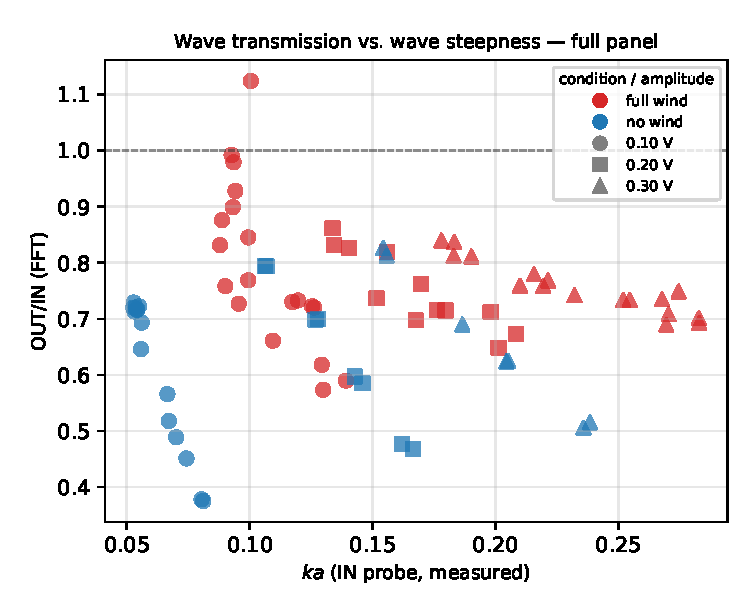
\includegraphics[width=\linewidth]{FIGURES/ch05_damping_ka_full.pdf}
  \caption{
    % TODO: write caption
  }
  \label{fig:ch05_damping_ka}
\end{figure}
